%"runningheads" enables:
%  - page number on page 2 onwards
%  - title/authors on even/odd pages
%This is good for other readers to enable proper archiving among other papers and pointing to content.

%Even though `american`, `english` and `USenglish` are synonyms for babel package (according to https://tex.stackexchange.com/questions/12775/babel-english-american-usenglish), the llncs document class is prepared to avoid the overriding of certain names (such as "Abstract." -> "Abstract" or "Fig." -> "Figure") when using `english`, but not when using the other 2.
\documentclass[runningheads,a4paper]{llncs}
\usepackage[english]{babel}

%better font, similar to the default springer font
%cfr-lm is preferred over lmodern. Reasoning at http://tex.stackexchange.com/a/247543/9075
\usepackage[%
rm={oldstyle=false,proportional=true},%
sf={oldstyle=false,proportional=true},%
tt={oldstyle=false,proportional=true,variable=true},%
qt=false%
]{cfr-lm}
%
%if more space is needed, exchange cfr-lm by mathptmx
%\usepackage{mathptmx}

\usepackage{graphicx}

%extended enumerate, such as \begin{compactenum}
\usepackage{paralist}

%put figures inside a text
%\usepackage{picins}
%use
%\piccaptioninside
%\piccaption{...}
%\parpic[r]{\includegraphics ...}
%Text...

%Sorts the citations in the brackets
%\usepackage{cite}

\usepackage[T1]{fontenc}

%for demonstration purposes only
\usepackage[math]{blindtext}

%for easy quotations: \enquote{text}
\usepackage{csquotes}

%enable margin kerning
\usepackage{microtype}

%tweak \url{...}
\usepackage{url}
%nicer // - solution by http://tex.stackexchange.com/a/98470/9075
\makeatletter
\def\Url@twoslashes{\mathchar`\/\@ifnextchar/{\kern-.2em}{}}
\g@addto@macro\UrlSpecials{\do\/{\Url@twoslashes}}
\makeatother
\urlstyle{same}
%improve wrapping of URLs - hint by http://tex.stackexchange.com/a/10419/9075
\makeatletter
\g@addto@macro{\UrlBreaks}{\UrlOrds}
\makeatother

%diagonal lines in a table - http://tex.stackexchange.com/questions/17745/diagonal-lines-in-table-cell
%slashbox is not available in texlive (due to licensing) and also gives bad results. This, we use diagbox
%\usepackage{diagbox}

%required for pdfcomment later
\usepackage{xcolor}

% new packages BEFORE hyperref
% See also http://tex.stackexchange.com/questions/1863/which-packages-should-be-loaded-after-hyperref-instead-of-before

%enable hyperref without colors and without bookmarks
\usepackage[
%pdfauthor={},
%pdfsubject={},
%pdftitle={},
%pdfkeywords={},
bookmarks=false,
breaklinks=true,
colorlinks=true,
linkcolor=black,
citecolor=black,
urlcolor=black,
%pdfstartpage=19,
pdfpagelayout=SinglePage,
pdfstartview=Fit
]{hyperref}
%enables correct jumping to figures when referencing
\usepackage[all]{hypcap}

%enable nice comments
\usepackage{pdfcomment}
\newcommand{\commentontext}[2]{\colorbox{yellow!60}{#1}\pdfcomment[color={0.234 0.867 0.211},hoffset=-6pt,voffset=10pt,opacity=0.5]{#2}}
\newcommand{\commentatside}[1]{\pdfcomment[color={0.045 0.278 0.643},icon=Note]{#1}}

%compatibality with TODO package
\newcommand{\todo}[1]{\commentatside{#1}}

%enable \cref{...} and \Cref{...} instead of \ref: Type of reference included in the link
\usepackage[capitalise,nameinlink]{cleveref}
%Nice formats for \cref
\crefname{section}{Sect.}{Sect.}
\Crefname{section}{Section}{Sections}

\usepackage{xspace}
%\newcommand{\eg}{e.\,g.\xspace}
%\newcommand{\ie}{i.\,e.\xspace}
\newcommand{\eg}{e.\,g.,\ }
\newcommand{\ie}{i.\,e.,\ }

%introduce \powerset - hint by http://matheplanet.com/matheplanet/nuke/html/viewtopic.php?topic=136492&post_id=997377
\DeclareFontFamily{U}{MnSymbolC}{}
\DeclareSymbolFont{MnSyC}{U}{MnSymbolC}{m}{n}
\DeclareFontShape{U}{MnSymbolC}{m}{n}{
    <-6>  MnSymbolC5
   <6-7>  MnSymbolC6
   <7-8>  MnSymbolC7
   <8-9>  MnSymbolC8
   <9-10> MnSymbolC9
  <10-12> MnSymbolC10
  <12->   MnSymbolC12%
}{}
\DeclareMathSymbol{\powerset}{\mathord}{MnSyC}{180}

% correct bad hyphenation here
\hyphenation{op-tical net-works semi-conduc-tor}

\begin{document}

%Works on MiKTeX only
%hint by http://goemonx.blogspot.de/2012/01/pdflatex-ligaturen-und-copynpaste.html
%also http://tex.stackexchange.com/questions/4397/make-ligatures-in-linux-libertine-copyable-and-searchable
%This allows a copy'n'paste of the text from the paper
\input glyphtounicode.tex
\pdfgentounicode=1

\title{Collecting operator-client conversation aligned with knowledge-base queries}
%If Title is too long, use \titlerunning
%\titlerunning{Short Title}

% %Single insitute
% \author{Ond\v{r}ej Pl\'{a}tek \and Filip Jur\v{c}\'{i}\v{c}ek}
% %If there are too many authors, use \authorrunning
% %\authorrunning{First Author et al.}
% \institute{Charles University in Prague, Faculty of Mathematics and Physics \\
% Insitute of Formal and Applied Linguistics \\
% Malostransk\'{e} n\'{a}m\v{e}st\'i 25, 11800 Praha 1, Czech Republic \\
% \email{\{oplatek,jurcicek\}@ufal.mff.cuni.cz}}

%Multiple insitutes
%Currently disabled
%
% \iffalse % FIXME enable for blind review and ucomment Single institute with filled values 
\iftrue % FIXME enable for blind review and ucomment Single institute with filled values 
%Multiple institutes are typeset as follows:
\author{Firstname Lastname\inst{1} \and Firstname Lastname\inst{2} }
%If there are too many authors, use \authorrunning
%\authorrunning{First Author et al.}

\institute{
Insitute 1\\
\email{...}\and
Insitute 2\\
\email{...}
}
\fi
			
\maketitle

\begin{abstract}
    This paper presents a novel datasets for training end-to-end task oriented conversational agents.
    The dataset contains task oriented conversation between an operator, a task expert, and a client who is seeking information about the task along with records of data base API calls of the operator, which capture the distilled meaning of the user query.
    The data base calls represent not only instantiation of user wishes but also, when evaluated against the database determine the answer from the database, which were used by the operator to provide requested information to the client. 
    We expect that this additional supervision of recording database interaction will provide enough information so the task of the conversation can be understood and behaviour of the interlocutors reconstructed by software agents.
    The dataset was collected using crowdsourcing in offline setting, where each contributor played role either of an operator or a client and contributed single utterance.
    The quality of the data were enforced by mutual control among contributors and manually verified on random sub-sample.
    The dataset is available for download under the Creative Commons 4.0 BY-SA license.
\end{abstract}

\keywords{task-oriented dialogue, end-to-end, dataset}

%%%%%%%%%%%%%%%%%%%%%%%%%%%%%%%%%%%%%%%%%%%%%%%%%%%%%%%%%%%%%%%%%%%%%%%%%%%%%%%
\section{Introduction}\label{sec:intro}
%%%%%%%%%%%%%%%%%%%%%%%%%%%%%%%%%%%%%%%%%%%%%%%%%%%%%%%%%%%%%%%%%%%%%%%%%%%%%%%
We present a new dataset of human-human task-oriented conversation in domain of Cambridge restaurant services targeted for supervised training of autonomous systems to play role of the operator which provides information about the restaurants to clients.
In contrast to previously released datasets, our datasets contains easy to obtain high-quality transcriptions of the client and operator actions during conversations.
We introduce a~very little overhead by collecting data base calls in addition to the transcription of the conversation. 
In fact, we mimic very closely a~real situation in call centers where operators searches for answers through database user interface. 
On the other hand, just logging the calls to the task database provide us with information of the similar quality as it is contained in manually annotated dialogue state, just not annotated incrementally after each turn.
Tracking the database calls in task oriented systems together with conversation transcription should not introduce much overhead during data collection, but should presumably boost end-to-end conversational agent as much as annotated dialogue state when training with such data.

Current Spoken Dialogue Systems (SDS) are either handcrafted and use no training data\cite{alex},\cite{todo}, but require non-trivial amount of expert work, or are gradually improved from initial policy through live user interaction\cite{Pomdp-young,gasix}, and lately are trained using supervised learning typically in end-to-end manner\cite{Wen2016,Williams2016}.\footnote{The~work of \cite{Williams2016} also fine tuned the conversation with reinforcement learning after the supervised-learning stage.}
The reinforce learning on one hand need just collect enough live user conversation without any transcription with the exception of explicit feedback at the end of each dialogue, but because the feedback signal is typically rather noise and delayed one require thousands of live conversations to improve rather simple policy.\cite{gasic}
The supervised-learning methods greatly reduced the number of conversation needed for training reasonable policy to few hundreds\cite{Wen2016}, but require annotation for all components used the dialogue which so far included at least a dialogue state\cite{Wen, his}.
Since the dialogue state is simplification of dialogue history and has no broadly-accepted form, it is very expensive to collect such annotated data because the dialogue state typically differs among domains and its structure is hard to explain to annotators.
In this paper, we focus on collecting supervised training set with rich enough annotation so the supervised models similar to~\cite{Wen2016} can be trained with few hundreds of dialogues, but the annotation of dialogues are much easier to collect.

We believe that the present dataset can be used for first experiments for end-to-end systems using supervised learning without annotated dialogue state.
The resulting systems should be able to roughly compare to systems trained on datasets with \cite{dstsc2, dstc3} dialogue state annotation because the same settings, i.e.\ database and task, for data collection.
Despite the fact, we collected human-to-human dialogues on known task of Cambridge restaurant domains the data-collecting method is completely domain and language independent.

The paper is structured as follows:
XY

% \section{End-to-end training of dialogue systems}
% \label{sec:training}

\section{Supervised feedback for task-oriented dialogue}
\label{sec:repre}
Traditionally, the dialogue systems are designed as pipelines of components, i.e.\ language understanding (LU) unit, dialogue tracker (DT), dialogue manager (DM) and natural language generator (NLG) for chat-based conversational agents.
If one want to use speech-to-speech conversational agent the 1-best ASR hypothesis can be used as input for LU unit and the NLG can be easily modified so its output is convenient for text-to-speech (TTS) unit which need to appended to the pipeline.

We focus on preparing training data so the LU, DT, DM and NLG components of dialogue system can be trained using such data.
The TTS and the ASR modules are typically trained with much more data and such data sets are out of scope of this paper.

It was shown that few hundreds of annotated domain specific conversation is needed for training relatively well performing LU~\cite{Alex} as well as Dialogue State Tracking~\cite{todo-Young?} components.
The work of~\cite{dusek} and~\cite{Marraise} showed that also several hundreds of conversations with appropriate annotation is needed for training usable NLG unit on simple domains.
Even the crucial task of action selection with reward provided only at the end of dialogue can be trained using POMDP dialogue manager and few thousands conversations~\cite{Gasic}.

A~novel work of~\cite{Wen} showed that only XY conversation annotated with just at dialogue state level is needed for training the whole end-to-end system performing the task of summarizing the dialogue history and reply planning and generation.
Consequently, we believe that end-to-end systems even with latent variables can be trained using few hundreds conversation if additional supervision in the form of simple annotation is used for narrow goal-oriented domains such as~\cite{Wen} domain or Cambridge restaurant domain~\cite{DSTC2}.

We note that on one hand further annotation of dialogue conversation may help to train the models faster, but simply collecting more data is typically more beneficial even with less annotation for models which does not require such annotation.
As a consequence, we see work of~\cite{Wen},~\cite{Borders} and~\cite{Williams} as great step forward since there work use annotation on dialogue state level or even no annotation for training dialogue agents.

On the other hand, we believe that annotating a dialogue state according to expert-handcrafted ontology is both artificial and still very labour intensive data collection task, so our work aim at collecting conversation with lighter but more easier to get annotations.
We suppose that a task-oriented  domain is defined by a task database e.g. in the Cambridge restaurant domain by database containing information about restaurants
We further suppose that there two roles in the conversation a {\it client} and a {\it operator}.
Typically, one wants to train a system which replaces the {\it operator} who is the domain expert.
{\it Clients} seek information stored in the database and use the system instead of human operator to obtain desired information.
In order to collect cheap high quality training data conversation one can record conversation between human operator and human clients.
Typically, the operator is provided with interface to the database so it can quickly find relevant information and play the role of domain expert.
We suggest to collect the operator's database calls with its arguments instead of dialogue state annotation after each turn.

The calls' to the database when call completely represents the client intention which is the purpose of the dialogue state.
On the other, the database calls are not present in every turn and thus by logging only the calls one loses a possibility to track partially filled client intention.
We argue that in high quality human-human conversation there is a minimum turns which are related to the domain and do not contain calls to the database as demonstrated in~Section~\ref{sec:props}.

\section{Dataset Collection Process}
\label{sec:collection}

Our data collection processed aimed at collecting natural conversation in the well defined domain.
We selected well studied Cambridge restaurant domain since the previous dataset~\cite{dstc1, dstc2, dstc3} in that domain demonstrated that a meaningful and not too long conversation can be held in the domain.
Also it was proven that the domain is on one hand difficult enough that even the state-of-the art systems does not reach human-level performance in the role of the operator and on the other hand numerous systems~\cite{young, gasic, Wen} demonstrated that are able to provide information to the clients most of the time.

We defined our domain by choosing a database from Dialogue State Tracking Challenge 2 (DSTC2)~\cite{dstc2} and explaining the interlocutors that there two roles a client and a operator.
For each conversation we determined goals for the client and provided the database for the operator.
We used the CrowdFlower (CF) crowdsourcing platform to collect the conversations.

We first describe the database which defines our domain in~Section~\ref{sec:db}.
Then we describe how the hired workers used our interface for playing either client or operator roles in~Sections~\ref{sec:client}and~\ref{sec:operator}.
Finally, in~Section~\ref{sec:async} we describe how we collected conversations one response at a time without connecting the interlocutors in real-time. 

\subsubsection{Domain database}
\label{sec:db}

We used exactly the same database as provided for the DSTC2 challenge.
The database contains information about 107 restaurants and their properties stored in the columns:

% \begin{itemize}
\begin{inparaenum}
    \item name (107),
    \item price range (3?),
    \item area (4),
    \item food (20?),
    \item address (90?),
    \item phone (90?),
    \item postcode (90?).
\end{inparaenum}
% \end{itemize}

We include the size of the vocabulary in brackets for each column.
The address or the postcode are unique for each restaurant but are sometimes missing, but the name of the restaurant is always known. 
There typically multiple restaurant with the same price range, area, or food type property.
These properties are sometimes unknown as well.

We use the database to generate the clients goals as demonstrated in~Figure~\ref{fig:client}, but only the operator is able to search the database (see~Figure~\ref{fig:operator}).

\subsubsection{Client interface}
\label{sec:client}

The client is given a goal to request provided information from the operator.
He may choose not to seek the goal immediately but submit more appropriate response such as greeting first.
The goals for the client are presented to the CF workers gradually and may contradict each other.
For example, the client may at first want a Chinese food, but later it changes her mind and wants to find restaurant serving British food.

Before submitting a reply the client is instructed to read the dialogue history and marked the goals which were presented to the operator.
The worker in the role of client is paid for each submitted response.

\begin{figure}
\begin{center}
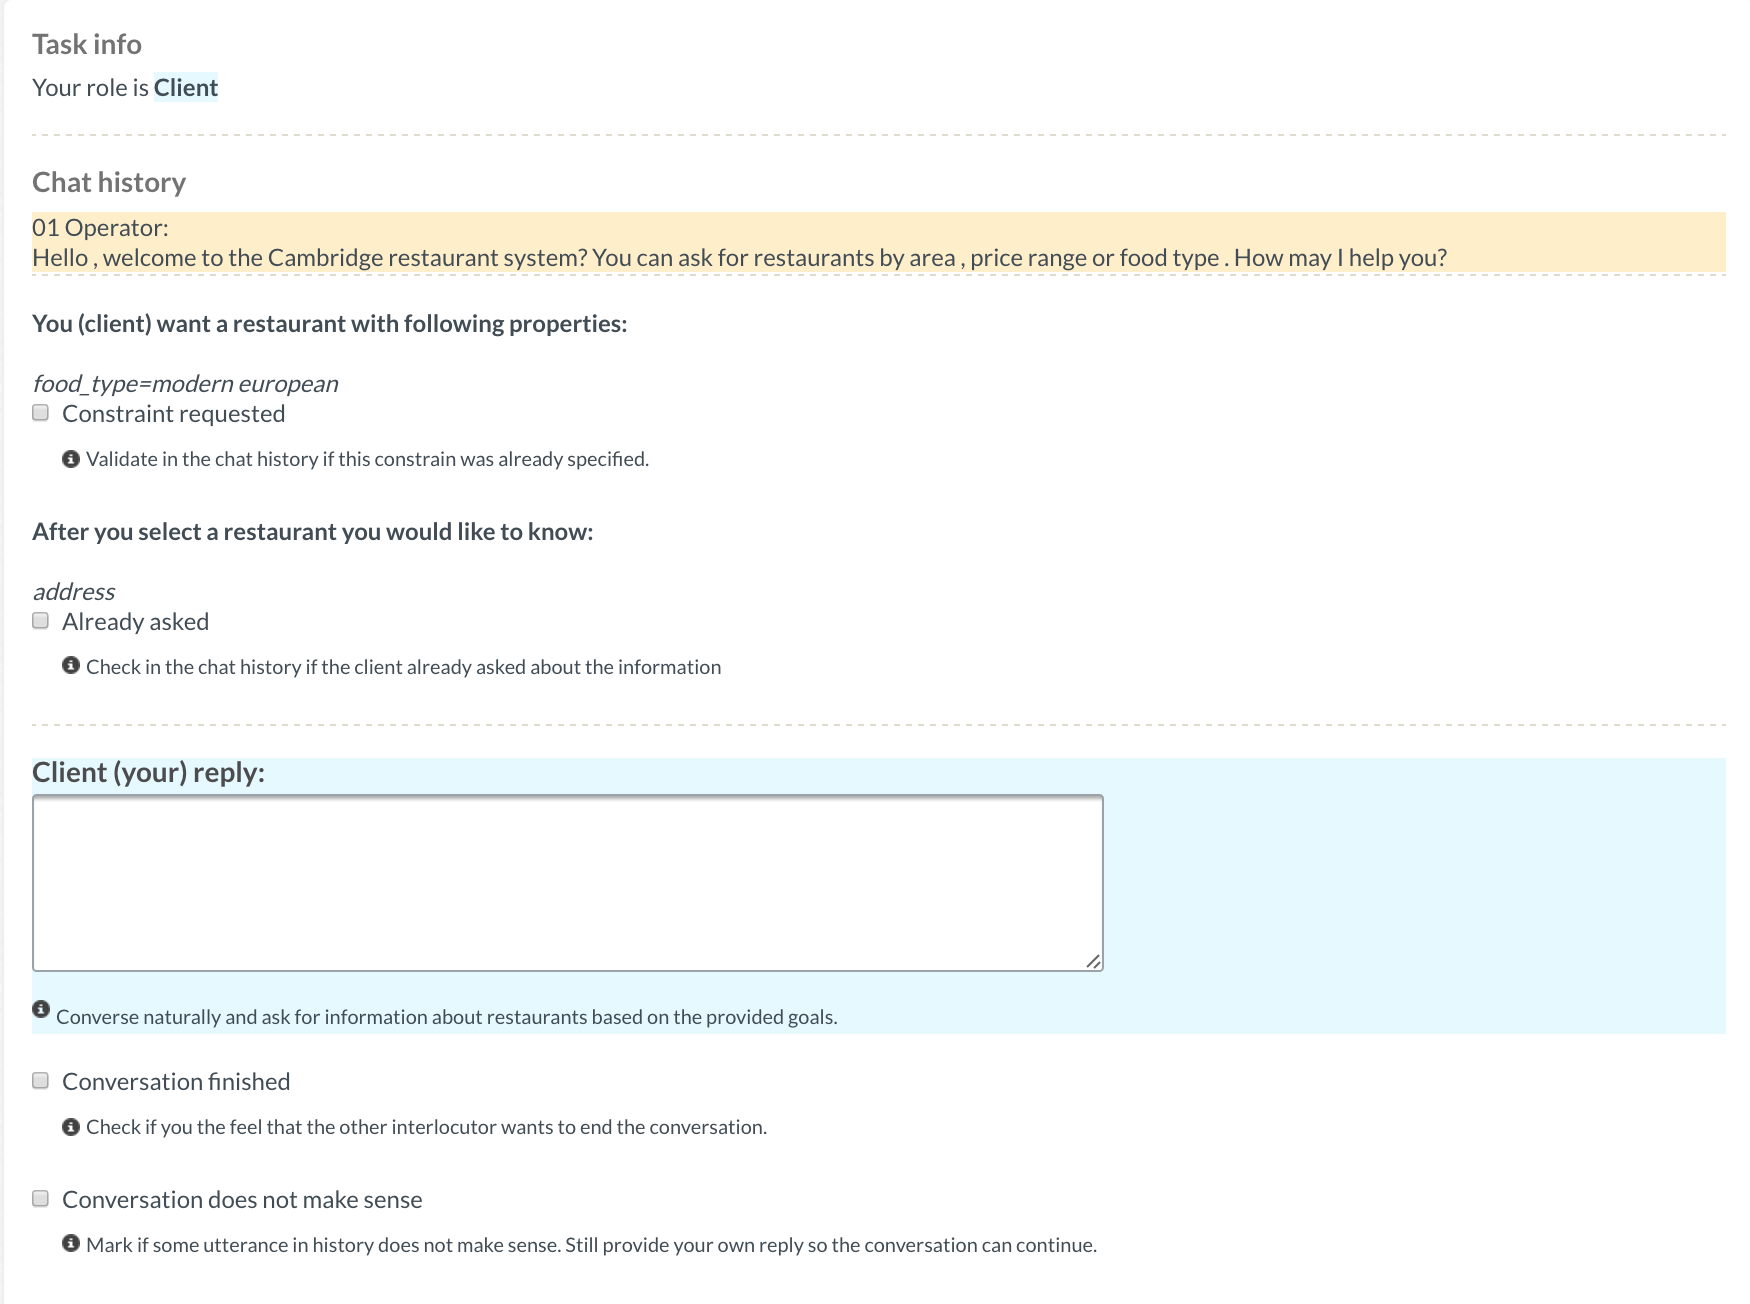
\includegraphics[height=25em]{gui-annotators-client}
\caption{Client annotation interface}
\end{center}
\vspace{-0.80em}
\label{fig:client}
\end{figure}

\subsubsection{Operator database}
\label{sec:operator}
The operator is asked to politely reply the clients needs according the information stored in the database.
In order to provide the informations to clients the operator uses the DB interface depicted in~Figure~\ref{fig:operator}.
Her or she filters the restaurants using a full text search on the database.
The content of the database is intentional hidden if no filter is specified so the filter has to be used.
The CF workers are also instructed also explicitly mark the rows of the restaurants about which provide the information in their answer.

\begin{figure}
\begin{center}
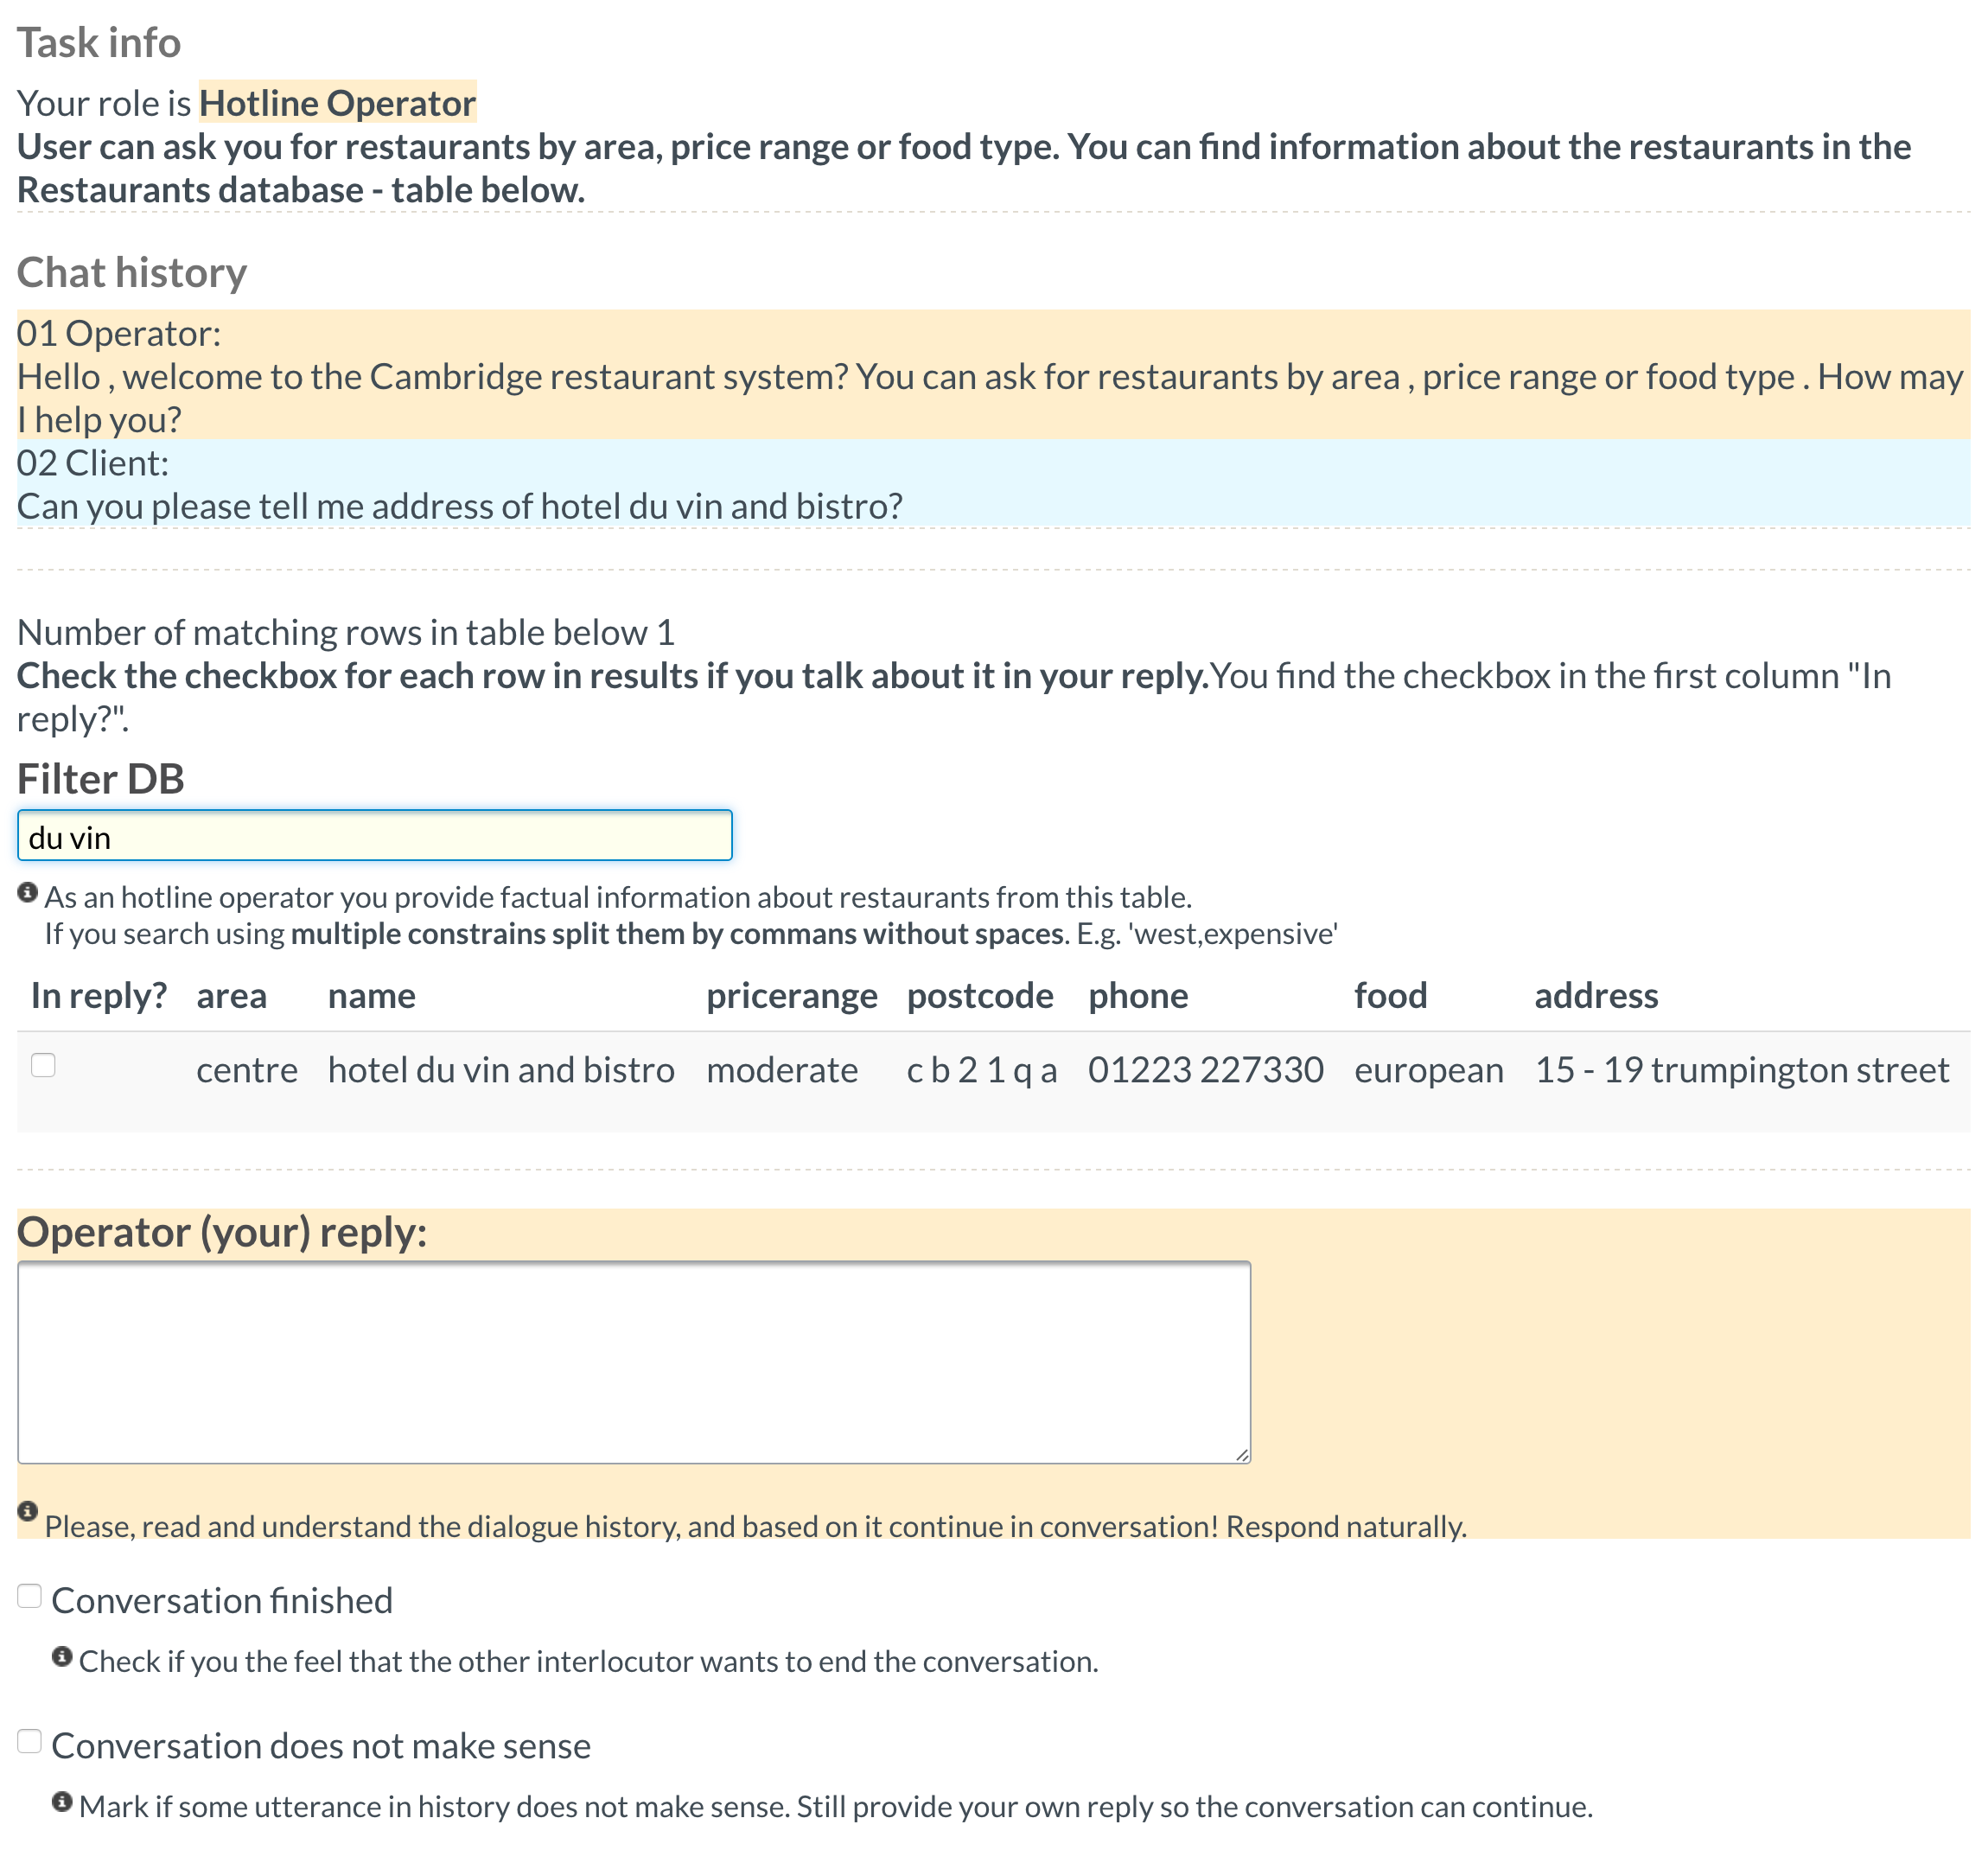
\includegraphics[height=25em]{gui-annotators-system}
\caption{Operator annotation interface}
\end{center}
\vspace{-0.80em}
\label{fig:operator}
\end{figure}

\subsubsection{Asynchronous collection without real-time responses}
\label{sec:async}
We design the crowdsourcing jobs so the CF contributors are able to work independently to each other.
One conversation is collected through out several rounds of jobs.
The roles of client and operator take turns as sets of partial conversations are submitted for collecting a single new response.
As a consequence, multiple contributors participate in submitting responses for single conversation for both roles.

Each utterance in conversation is submitted by different contributor, so contributors need to read carefully the dialogue history to understand the conversation before submitting their response.
The workers are able to mark dialogues which does not make sense and thus they self-assess quality of the conversations.
Note also that the conversation are typically rather short taking only from {\bf TODO} four to six turns including first turn with greetings.
The contributors mark the conversations as finished if they have no more goals to fulfill and all the goodbyes were said.

We bootstrap the conversation with either with an operators introduction "{\it Hello , welcome to the Cambridge restaurant system? You can ask for restaurants by area , price range or food type . How may I help you?}" and the first contributors play role of the client or we bootstrap the conversation full turn with aforementioned operators utterance and clients greeting e.g. "Hi" so the contributors play role of the operator.

To avoid poor language level of English we restricted the CF worker to English-speaking countries.
We further perform heuristically check for too trivial answers and we added ability to the CF workers to rate each others submission.
It help us filter low quality submission, but more importantly it motivated workers not to cheat. 

% TODO describe how we started with 5 bootstrapped conversation with client role 5 without it and then mixed the partial with new one and resubmit them until the first conversations were marked as finished.


\section{Dataset Properties}
\label{sec:props}

We collected XY conversation with average length ZY.
During an average conversation 2.4-TODO tasks are requested and answered.
Typically in 65-TODO \% case the conversation is ended by the client

\begin{table}
\begin{center}
\begin{tabular}{lrr}
\hline
Set   & \# Dialogues & \# Turns \\
\hline
% Joint  &  todo &  todo \\
% /a/SSD/oplatek/e2end/log/2016-06-08-17-31-38.400-dstc-INDEP_labels-d0.7-w100-e100/
% /a/SSD/oplatek/e2end/log/TEST-ORIGINAL-2016-06-08-17-31-38.400dstc-INDEP_labels-d0.7-w100-e100-reward-0.9080-step-0036224
Train  &   ? & ? \\
Dev &   ? & ? \\
Test &   ? & ? \\
\hline
\end{tabular}
\caption{Accuracy on development and test set}
\vspace{-2em}
\end{center}
\label{tab:props}
\end{table}

During the data collection process we discarded roughly 40-TODO \% of conversation in total.


\section{Related Work}
\label{sec:related}

Our work is closely related  to work of~\cite{dstc1, dstc2, dstc3} in the sense that the conversation are held in the same domain.
On the other hand, the collection process differs substantially because we do not use any artificial system and rather we focus on collecting high quality human conversations. In addition, in our work we do not collect complicated annotation on LU and DST level as it was previously done on DST challenges.

A very relevant work of~\cite{Wen} collected human-human dialogues in similar domain to the Cambridge domain according their description.
Their dataset is not yet published so we compare only with their statistics.
The dataset is of similar size and used very similar collection scheme where the Amazon Mechanical Turk workers submitted one reply at a time without being connected to each other in real-time.

Another line of research~\cite{mirek-interactive} used CF to collect human-human conversation for interactive-learning dataset.
However, the collected dialogues were later annotated by expert annotators which goes directly against our intentions to avoid any expensive annotations.

There is tremendous amount of work describing Wizard of Oz experiments~\cite{walker,schlangen,someone} which either focused on studying linguistic properties of dialogues, evaluated proof of concept or even collected bootstrap training data, but definitely, according our knowledge, do not use cheap crowdsourcing workers to collect a~full training dataset.

\section{Conclusion and Future work}
\label{sec:conc}
We present a new human-human dialogue dataset with annotation of user intension in form of their database calls.
We also introduced a novel data collection setting which resembles work of operators in call centers and introduce minimum overhead to crowdsourcing workers.
The collected dialogues are published under Creative Commons 4.0 BY-SA license on available to download at {\it anonymised}.  % lindat\footnote{todo where}.

We plan to increase the number of collected dialogues till the camera ready deadline to XYZU.
We intend to use the dataset to train and evaluate an~end-to-end conversational model which uses only the database calls as additional supervision to the recorded responses. 

\subsubsection*{Acknowledgments}
We would like to thank Ond\v{r}ej Du\v{s}ek for useful comments.
This research was partly funded by the Ministry of Education, Youth and Sports of the Czech Republic under the grant agreement LK11221, core research funding, grant GAUK 1915/2015, and also partially supported by SVV project number 260 333. 
We gratefully acknowledge the support of NVIDIA Corporation with the donation of the Tesla K40c GPU used for this research.
Cloud computational resources were provided by the MetaCentrum under the program LM2010005 and the CERIT-SC under the program Centre CERIT Scientific Cloud, part of the Operational Program Research and Development for Innovations, Reg.\ no. CZ.1.05/3.2.00/08.0144.

% ``something in quotes'' using plain tex or use \enquote{the enquote command}.
% cref Demonstration: Cref at beginning of sentence, cref in all other cases.
%
% \Cref{fig:simple} shows a simple fact, although \cref{fig:simple} could also show something else.
%
% \Cref{tab:simple} shows a simple fact, although \cref{tab:simple} could also show something else.
%
% \Cref{sec:intro} shows a simple fact, although \cref{sec:intro} could also show something else.
%
% Brackets work as designed:
% <test>
%
% The symbol for powerset is now correct: $\powerset$ and not a Weierstrass p ($\wp$).
%
% \begin{inparaenum}
% \item All these items...
% \item ...appear in one line
% \item This is enabled by the paralist package.
% \end{inparaenum}
% In the bibliography, use \texttt{\textbackslash textsuperscript} for ``st'', ``nd'', ...:
% E.g., \enquote{The 2\textsuperscript{nd} conference on examples}.
% When you use \href{http://www.jabref.org}{JabRef}, you can use the clean up command to achieve that.


% Winery~\cite{Winery} is graphical \commentontext{modeling}{modeling with one \enquote{l}, because of AE} tool.
%%%%%%%%%%%%%%%%%%%%%%%%%%%%%%%%%%%%%%%%%%%%%%%%%%%%%%%%%%%%%%%%%%%%%%%%%%%%%%%
\bibliographystyle{splncs03}
\bibliography{paper}

All links were last followed on June 28, 2016.
%%%%%%%%%%%%%%%%%%%%%%%%%%%%%%%%%%%%%%%%%%%%%%%%%%%%%%%%%%%%%%%%%%%%%%%%%%%%%%%

\end{document}
